\chapter{User study} \label{chapter3}

Finding the right approach to our implementation requires, first and foremost, collecting feedback and insights from the students of the \textbf{ACS}. In the end, we do not intend to have only a functioning product but to deploy a feature that students could use on a daily basis. Therefore, our goals for this user study are:

\begin{itemize}
    \setlength{\topsep}{0.5pt}
    \setlength{\itemsep}{0.5pt}
    \setlength{\parsep}{0.5pt}
    \item to understand how students are impacted by the problem of navigating multiple information sources
    \item to analyze how students use different platforms to retrieve their data
    \item to have a clear view of what features would best fit our students' needs
\end{itemize}

\section{Methods} \label{3:methods}

We employed two different methods for our research process: a \textbf{survey} sent to students of all years from \textbf{ACS}, and \textbf{discussions} with key student figures who hold representative functions and are well aware of our faculty's present problems. Due to the recent pandemic situation \footnote{https://en.wikipedia.org/wiki/COVID-19\_pandemic}, we conducted our research process integrally via online means. While our discussions were held on social networking platforms, our survey was conducted via \textit{Google Forms} \footnote{https://docs.google.com/forms} and distributed to several students \textit{Whatsapp} \footnote{https://web.whatsapp.com/} groups.

~
We decided to hold our discussions first to get a general view of our problem and better formulate our survey questions later. When discussing with these individuals, we tried to formulate our problem and ask for some general opinions about it. We intended to receive a general feel of how students are affected by the need to navigate several information platforms. Surprisingly, our discussions revealed that people at \textbf{ACS} had raised the issue of not having a centralized information channel before, but there had been no particular action on this matter.

~
Our survey was opened for an entire month in \textbf{December 2021} and received \textbf{112} total responses. Although Google Forms allows for visualizing data under different representations, we exported our results and used \textit{Python Matplotlib} \footnote{https://matplotlib.org/} and \textit{Seaborn} \footnote{https://seaborn.pydata.org/} to plot our information.

\section{Target audience} \label{3:audience}

We tried to target students from both the Bachelor's and Master's stages for our study. \textbf{ACS} currently has a four-year Bachelor's cycle and a two-year Master's cycle. Our results follow the distribution illustrated in figure \ref{3:fig:students_year_piechart}.

\begin{figure}[ht]
    \centering
         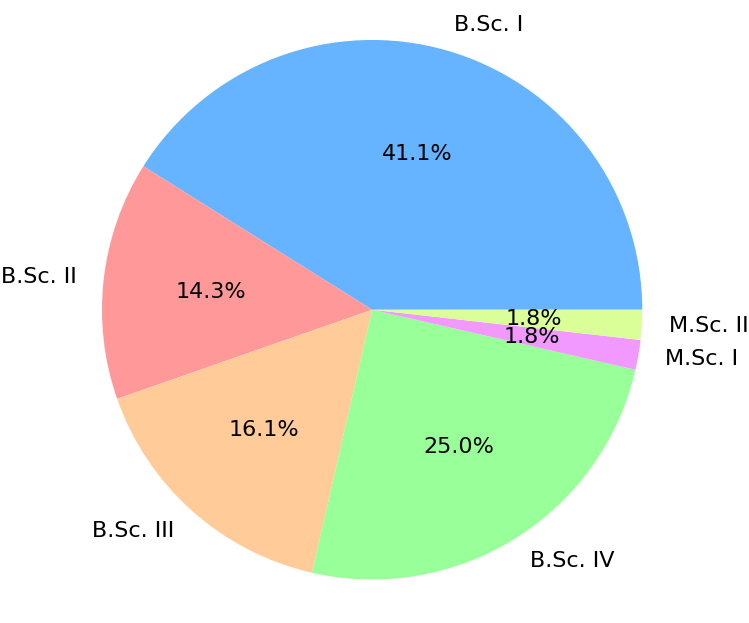
\includegraphics[height=0.35\textheight]{figures/charts/survey/survey-students-year-piechart.png}
    \caption{Students distribution by year}
    \label{3:fig:students_year_piechart}
\end{figure}

~

About \textbf{96.4\%} of all submissions came from undergraduate students, whereas \textbf{3.6\%} came from students enrolled at Master's degree. While most of the Bachelor's submissions came from first-year students, the Master's distribution is equal along the two-year cycle.

~
Concerning the demographics, we tried to analyze the distribution of students that hold any significant or representative role within their collective. Our results are illustrated by the following barchart \textbf{\ref{3:fig:students_representatives}}. Students were not limited to choosing only one role, and in practice, some students may have multiple representative roles. 
Results show that some 14\% of all students hold at least one position, 5\% may be involved in student organizations, and 1\% may be present in the Faculty Council.

\begin{figure}[ht]
    \centering
         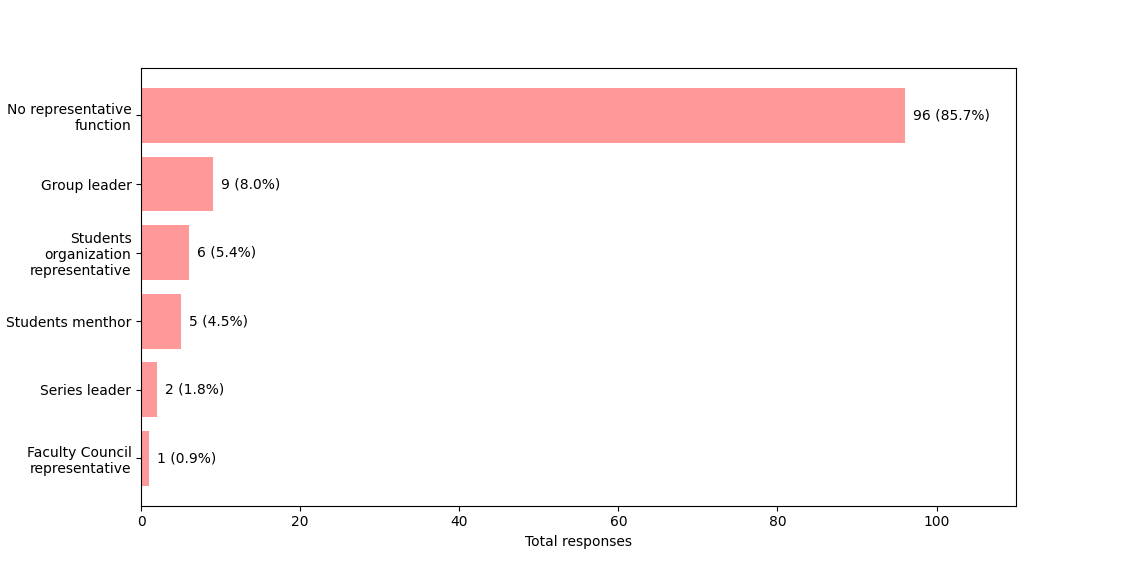
\includegraphics[height=0.35\textheight]{figures/charts/survey/survey-students-representatives-bar.png}
    \caption{Distribution of students in representative roles}
    \label{3:fig:students_representatives}
\end{figure}

Additionally, we tried to assess how involved students are in different student organizations and impressively, close to 50\% are present in at least one such association. The following chart \textbf{\ref{3:fig:students_organizations}} shows that almost half of all students combine faculty with extracurricular activities.

\begin{figure}[ht]
    \centering
         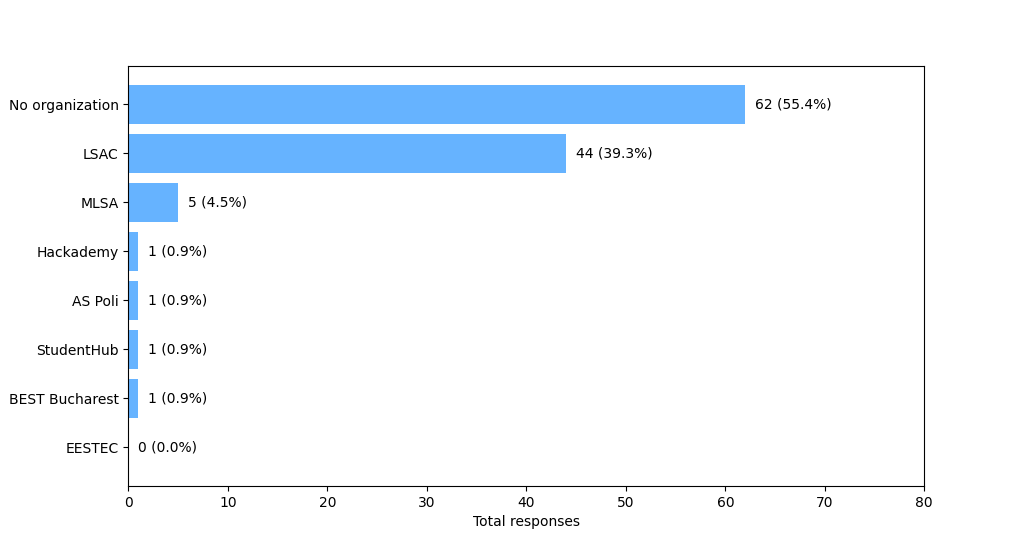
\includegraphics[height=0.35\textheight]{figures/charts/survey/survey-student-organizations-bar.png}
    \caption{Distribution of students involved in organizations}
    \label{3:fig:students_organizations}
\end{figure}

~
We concluded that our survey captured a good representation of the real-life demographics. While a small fraction of students (about 1/10 students) are involved in representative responsibilities, an impressive percentage is involved in student organisations or volunteer activities. Because not many Master's students completed the survey, we think our solution best fits the undergraduate group's needs. However, we are reasonably confident that it will positively impact the postgraduate students as well.

~

\section{Results} \label{3:results}

Following our survey, we tried to reach our goals mentioned in the opening of this chapter. We tried to provide a survey with clear questions and flexible answering methods, so that we capture as many details as possible about the relationship between students and their information sources.

\subsection{Student behaviour} \label{3:behaviour}

One of our questions focused on students' behaviour and how they collect their information. We listed the leading platforms for students at \textbf{ACS} and several resource categories. Our results consist of a heatmap \ref{3:fig:heatmap_behaviour} showing what platforms are most used for a specific resource category. 

\begin{figure}[ht]
    \centering
         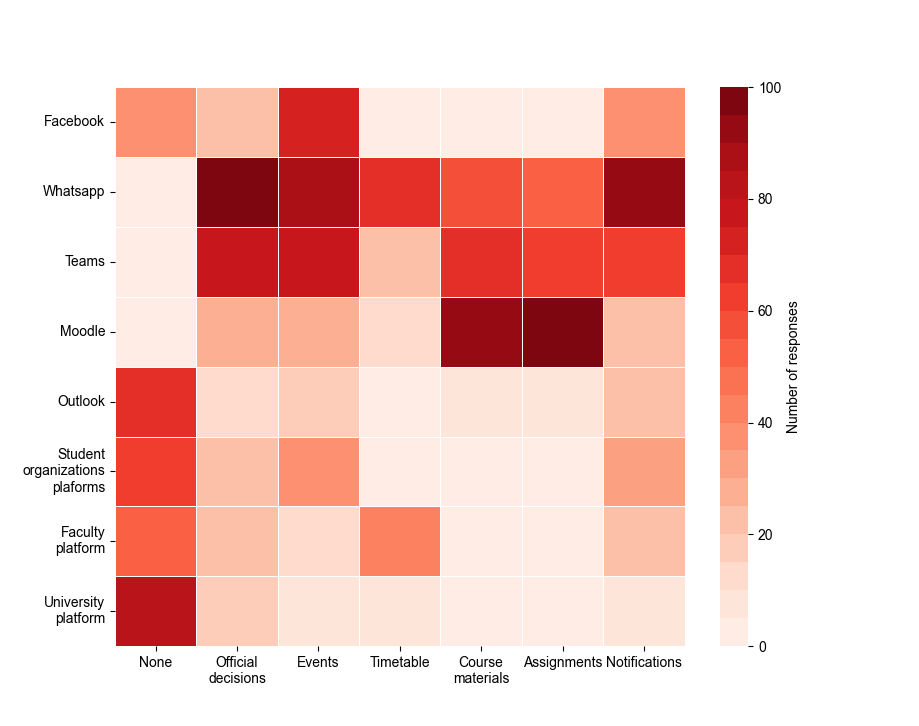
\includegraphics[height=0.55\textheight]{figures/charts/survey/survey-platforms-heatmap.png}
    \caption{Relationship between platform and searched resources}
    \label{3:fig:heatmap_behaviour}
\end{figure}

~
The majority of responses show that the official platforms (\textit{faculty}\footnote{https://acs.pub.ro/}, \textit{university}\footnote{https://upb.ro/}) are significantly less used in all categories in comparison to all the others. Survey shows that \textit{Whatsapp} is by far, the channel most used when it comes to students getting their information and resources. This result makes sense since chatting apps are faster and more efficient in terms of real-time communication, but these are not necessarily protected from spam and unregulated content. Since the break of the recent pandemic, all faculty-related activities have moved online on \textit{Teams}\footnote{https://www.microsoft.com/ro-ro/microsoft-teams/log-in} and survey shows that is heavily used by students. \textit{Moodle}\footnote{https://curs.upb.ro/2021/} remains specialized on assignments management, but tends to fail in other categories. Despite its convoluted nature, \textit{Facebook}\footnote{https://www.facebook.com/} remains one of students' favorite choice regarding events and faculty announcements.

~ 
As a special note, \textit{Outlook} is less relevant to students at \textbf{ACS} than the majority of other platforms. While other faculties tend to heavily make use of Outlook or any other mailing service (as mentioned in \textbf{chapter \ref{chapter2}}), students at \textbf{ACS} find it less important or visible when navigating their daily faculty content. We could argue that email is generally a powerful tool to push relevant content to people, but in this particular case, it fails to achieve its intended purpose.

~
Following this result, we could draw a few conclusions. First, students choose to stay informed on platforms that push content and activity constantly. Second, it could be argued that social networks and chatting apps significantly win because they have tailored apps for both desktop and mobile versions and more efficient UI/UX features. Finally, official platforms might lack popularity for many reasons. These may have a weak user interface that does not adhere to most modern standards, rare fresh content and little activity (such websites tend to work more as virtual panels rather than engaging platforms), and these lack a push-notification system.

\subsection{Problems} \label{3:problems}

Besides students' behaviour, we investigated what problems students deal with when they try to stay informed on a daily basis. We listed several common problems, and we had students give an appreciative score on how much that issue affects their information searching experience.

~
We had a five-step grading system: \textbf{Totally annoyed}, \textbf{Annoyed}, \textbf{Neutral}, \textbf{Relatively indifferent} and \textbf{Indifferent}. When putting all data together, we gave a specific score to each step, as shown in the figure \ref{3:fig:student_problems}.

\begin{figure}[ht]
    \centering
         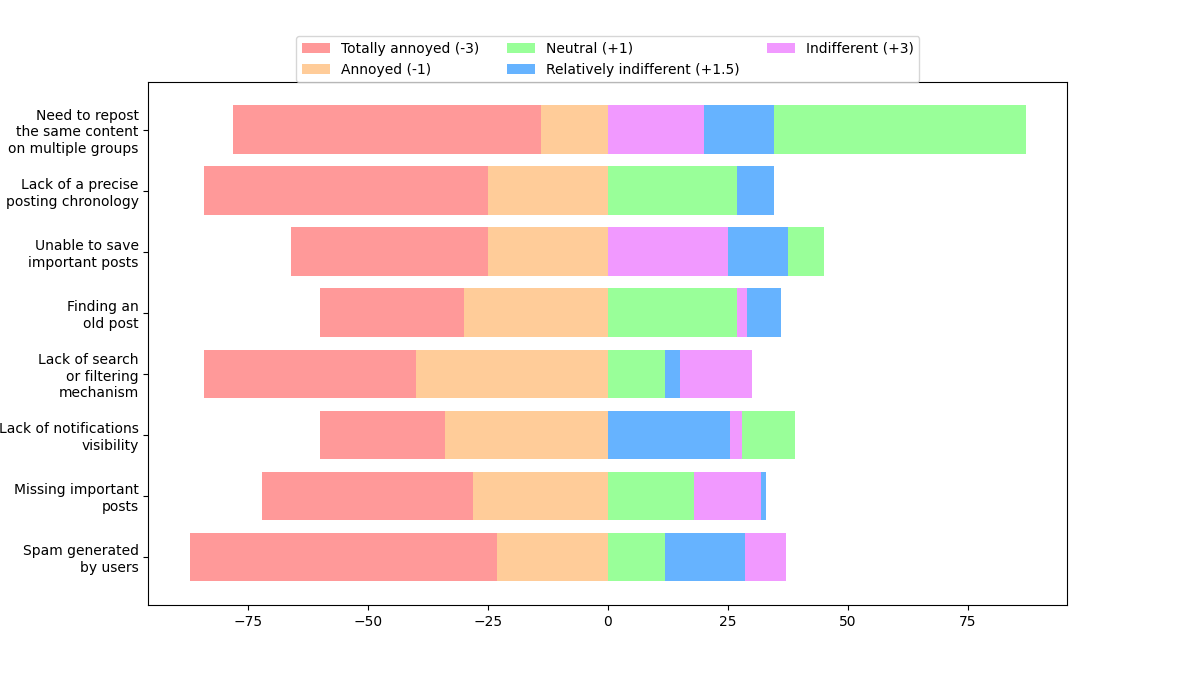
\includegraphics[height=0.42\textheight]{figures/charts/survey/survey-study-problems-stacked.png}
    \caption{Degree of impact for each problem}
    \label{3:fig:student_problems}
\end{figure}

~
The most adverse problems that students confront with are: the spam generated by users, the lack of a precise posting chronology and the lack of search or filtering mechanism.
Besides the usual spam, students point out that a clear disadvantage of navigating multiple platforms is the lack of organization and a standard format that would allow them to sort the content uniformly. A precise chronology or a filtering system are issues that should be considered when designing our solution.
The need to repost the same content to multiple groups is the most polarizing problem since equally as many students are disturbed as students who are indifferent to this issue. Finally, the lack of notifications visibility is surprisingly one of the least negative issues, but we argue that notifications still impact a lot the students' engagement factor.

~

Having a survey confirmation of what problems are the most priority to deal with, we can follow through and assess which features would best fit the students' needs.

\subsection{Solutions} \label{3:solutions}

For this evaluation, we proceeded similarly to the latest sub-chapter \ref{3:problems}. We listed several features and we had students grade them based on an intuitive five-grade scale: \textbf{Useless}, \textbf{Not so useful}, \textbf{Relatively useful}, \textbf{Useful} and \textbf{Very Useful}. Each grade was assigned a specific score, and by putting all data together, we obtained the following chart \ref{3:fig:solutions}:

\begin{figure}[ht]
    \centering
         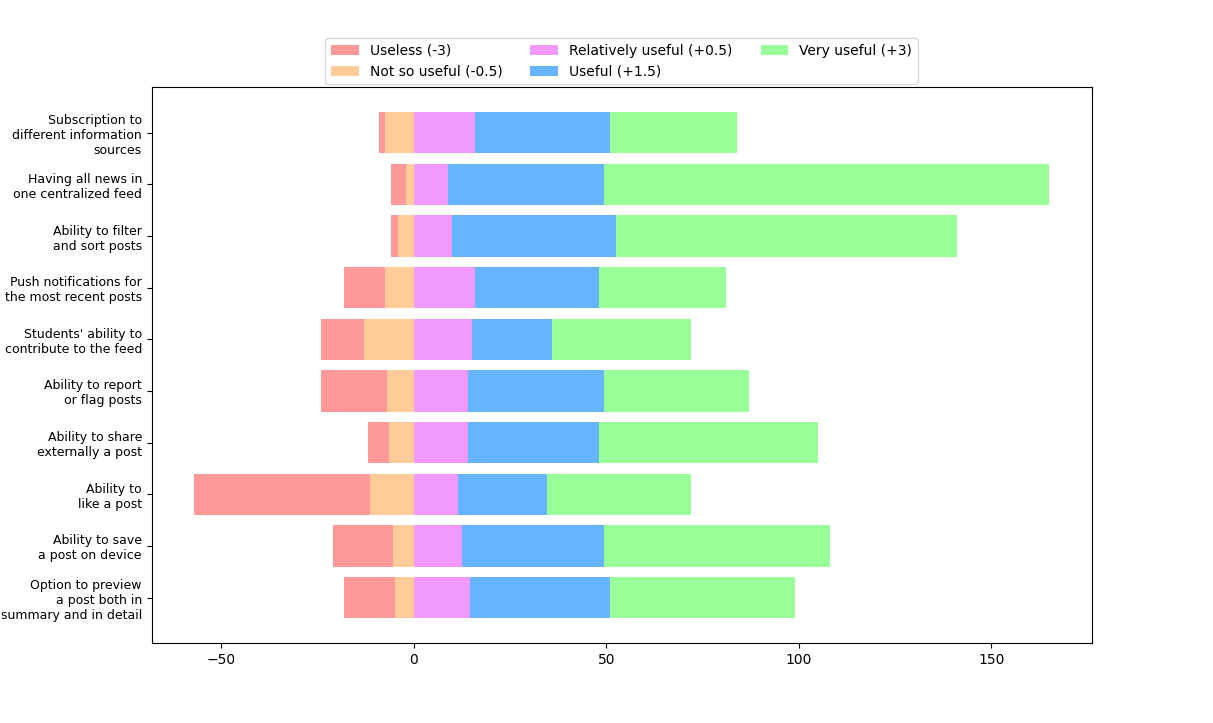
\includegraphics[height=0.42\textheight]{figures/charts/survey/survey-features-ranking-stacked.png}
    \caption{Degree of usefulness for each feature}
    \label{3:fig:solutions}
\end{figure}

~
The need to have all news in one centralized feed is undoubtedly the most requested feature with predominantly positive feedback. Second to this, the ability to filter and sort posts received great appreciation from students, and this result ties up naturally with the scores obtained in the previous chart \ref{3:fig:student_problems}. Moving forward, the following features received big scores as well and are worth taking into account when designing our news feed aggregator: the ability to share a post externally, the ability to save a post on the device, option to view a post both in summary and in details, push notifications, subscription to different information sources.

~
Interestingly, the ability to like a post received the most negative feedback. We could argue that such social actions (like, comments) characteristic of most extensive social networks are not appropriate to our use case. Although the students' ability to contribute to the feed received a similar positive score, we consider this feature to be necessary since, in the end, we want our feed to collect information from several sources, official and non-official, such as students. Nevertheless, having a system that carefully grants posting roles to individuals should strike the right balance between our goal and the students' feedback.